\subsection{Writing Applications and Services}

All applications are started under control of the Application Manager
and must implement the  Java interface \texttt{usr.applications.Application}.

\begin{lstlisting}[language=java,frame=single]
/**
 * An Application has is a Runnable object that has a managed lifecycle.
 */
public interface Application extends Runnable {
    /**
     * Initialize with some args
     */
    public ApplicationResponse init(String[] args);

    /**
     * Start an application. This is called before run().
     */
    public ApplicationResponse start();

    /**
     * Stop an application.
     * This is called to implement graceful shut down and cause run() to end.
     */
    public ApplicationResponse stop();
}
\end{lstlisting}

\noindent Notice that \texttt{Application} extends \texttt{Runnable},
so this means that applications must have a \texttt{run()} method.
This is where the \emph{main} body of the app resides.

The ApplicationResponse object has 2 fields: (i) a $boolean$
value to indicate if the app is progressing well, where $true$ means
success and $false$ mean failure, (ii) a message that may be passed
on.

If any of these methods returns an ApplicationResponse with a
$false$ value then the system will stop what it is doing, and clean up
the application context.

\subsubsection{An Example App -- Sending Data}

Here is an app that opens a Socket and sends datagrams.
When it is started it takes 3 arguments: an address to send to, a port
to send to, and a count of the number of datagrams.

\begin{lstlisting}[language=java,frame=single]
public class Send implements Application {
    Address addr = null;
    int port = 0;
    int count = 0;

    boolean running = false;
    DatagramSocket socket = null;
    
\end{lstlisting}


\noindent  The \texttt{init()} method is defined to process all the
arguments that are passed in.

\begin{lstlisting}[language=java,frame=single]
    public ApplicationResponse init(String[] args) {
        if (args.length == 3) {
            // try address
            try {
                addr = AddressFactory.newAddress(args[0]);

            } catch (Exception e) {
                return new ApplicationResponse(false, "UnknownHost " + args[0]);
            }

            // try port
            Scanner scanner = new Scanner(args[1]);

            if (scanner.hasNextInt()) {
                port = scanner.nextInt();
                scanner.close();
            } else {
            	scanner.close();
                return new ApplicationResponse(false, "Bad port " + args[1]);
            }

            // try count
            scanner = new Scanner(args[2]);

            if (scanner.hasNextInt()) {
                count = scanner.nextInt();
                scanner.close();
            } else {
            	scanner.close();
                return new ApplicationResponse(false, "Bad count " + args[2]);
            }

            // we got here ok so return true
            return new ApplicationResponse(true, "");

        } else {
            return new ApplicationResponse(false, "Usage: Send address port count");
        }
    }
\end{lstlisting}

\noindent If the application returns an ApplicationResponse with a
$true$ value then the system will progress to the \texttt{start()}
method.

In this case the application creates a new socket and connects to the
remote router. If the connect fails then the ApplicationResponse is
$false$ and the application will stop, otherwise it returns an
ApplicationResponse with $true$ and it progresses to the
\texttt{run()} method.

\begin{lstlisting}[language=java,frame=single]
    public ApplicationResponse start() {
        try {
            // set up socket
            socket = new DatagramSocket();

            socket.connect(addr, port);

        } catch (Exception e) {
            return new ApplicationResponse(false, "Cannot open socket " + e.getMessage());
        }

        running = true;

        return new ApplicationResponse(true, "");
    }
\end{lstlisting}

\noindent The \texttt{run()} method creates a new datagram and sends
it onwards.

\begin{lstlisting}[language=java,frame=single]
    public void run() {
        Datagram datagram = null;

        // a buffer for data
        byte [] buffer;

        // loop around        
        for (int i = 0; i < count; i++) {
            // Code to Fill the Buffer

            datagram = DatagramFactory.newDatagram(buffer);

            try {
                socket.send(datagram);

            } catch (Exception e) {
                if (socket.isClosed()) {
                    break;
                } else {
                    // maybe try again
                }
            }
        }
    }
\end{lstlisting}

\noindent Finally the \texttt{stop()} method is shown.
This method is called by the Application Manager when the Application
is terminated in some way, either by explicitly being stopped by a
REST API call or by shutting down the whole system.


\begin{lstlisting}[language=java,frame=single]
    public ApplicationResponse stop() {
        running = false;

        if (socket != null) {
            socket.close();
        }

        return new ApplicationResponse(true, "");
    }
\end{lstlisting}

\subsubsection{An Example App -- Receiving Data}

Here is an app that opens a Socket and receives datagrams.
When it is started it takes 1 argument, whic is the port to listen on.

\begin{lstlisting}[language=java,frame=single]
public class Recv implements Application {
    int port = 0;

    int count = 0;

    boolean running = false;
    DatagramSocket socket = null;

\end{lstlisting}

\noindent  The \texttt{init()} method is defined to process the
arguments that are passed in.

\begin{lstlisting}[language=java,frame=single]
    public ApplicationResponse init(String[] args) {
        if (args.length == 1) {
            // try port
            Scanner scanner = new Scanner(args[0]);

            if (scanner.hasNextInt()) {
                port = scanner.nextInt();
                scanner.close();
            } else {
            	scanner.close();
                return new ApplicationResponse(false, "Bad port " + args[1]);
            }

            return new ApplicationResponse(true, "");

        } else {
            return new ApplicationResponse(false, "Usage: Recv port");
        }
    }
    
\end{lstlisting}


\noindent Again, if the application returns an ApplicationResponse with a
$true$ value then the system will progress to the \texttt{start()}
method.

In this case the application creates a new socket and
$binds$ to the specified port.
If this fails then the ApplicationResponse is
$false$ and the application will stop, otherwise it returns an
ApplicationResponse with $true$ and it progresses to the
\texttt{run()} method.

\begin{lstlisting}[language=java,frame=single]
    public ApplicationResponse start() {
        try {
            // set up socket
            socket = new DatagramSocket();

            socket.bind(port);

        } catch (Exception e) {
            return new ApplicationResponse(false, "Cannot open socket " + e.getMessage());
        }

        running = true;

        return new ApplicationResponse(true, "");
    }

\end{lstlisting}


\noindent The \texttt{run()} method receives each datagram 
prints out some meta-data.

\begin{lstlisting}[language=java,frame=single]
    public void run() {
        Datagram datagram;

        try {
            while ((datagram = socket.receive()) != null) {

                System.out.print(count + ". ");
                System.out.print("HdrLen: " + datagram.getHeaderLength() +
                                 " Len: " + datagram.getTotalLength() +
                                 " Time: " + (System.currentTimeMillis() - 
                                                    datagram.getTimestamp()) +
                                 " From: " + datagram.getSrcAddress() +
                                 " To: " + datagram.getDstAddress() +
                                 ". ");

                byte[] payload = datagram.getPayload();

                if (payload == null) {
                    System.out.print("No payload");
                } else {
                    System.out.print(new String(payload));
                }
                System.out.println("");

                count++;
            }
        } catch (SocketException se) {
            System.out.println(se.getMessage());
        }
    }
    
\end{lstlisting}

\noindent Finally the \texttt{stop()} method is shown.
This method is called by the Application Manager when the Application
is terminated in some way, either by explicitly being stopped by a
REST API call or by shutting down the whole system.

\begin{lstlisting}[language=java,frame=single]
    public ApplicationResponse stop() {
        running = false;

        if (socket != null) {
            socket.close();
        }

        return new ApplicationResponse(true, "");
    }
\end{lstlisting}

\subsection{Writing Topology and Management Applications}

This section presents the ways of writing topology focused
applications and management
applications for VLSP.  Such applications can include scenarios such
as: (i) experiment setup, control, and execution; (ii) orchestration
strategies; (iii) dashboards; etc.




\subsubsection{VIM Client}

The Vim Client, \texttt{usr.vim.VimClient} is a Java wrapper
for the REST API, detailed in appendix \ref{chap:restapi}.
The VimClient methods are shown in detail in appendix \ref{chap:vimclient},
It is possible to write a Vim Client in any language, and we have
versions of them written in \texttt{clojure},  \texttt{Julia} and also
 \texttt{python}.

If you do not have VLSP Client yet, you can find the source on
\textit{gitlab} at

\code{https://gitlab.com/sclayman/vlsp-client}

 


In the following example we show how to use the VimClient to create a
virtual network.

\begin{figure}[ht!]
  \centering
  \resizebox{0.7\textwidth}{!}{%

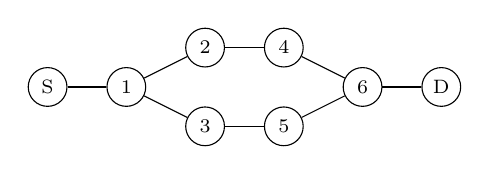
\begin{tikzpicture}%
  \node[circle,draw=black, fill=none, inner sep=0pt,
    minimum size=14pt, font=\scriptsize] (r1) at (1,0.5) {1};
      
  \node[circle,draw=black, fill=none, inner sep=0pt, 
    minimum size=14pt, font=\scriptsize]  (r2) at (2,1) {2};
  
  \node[circle,draw=black, fill=none, inner sep=0pt,
    minimum size=14pt, font=\scriptsize] (r3) at (2,0) {3};

  \node[circle,draw=black, fill=none,  inner sep=0pt,
    minimum size=14pt, font=\scriptsize] (r4) at (3,1) {4};

  \node[circle,draw=black, fill=none, inner sep=0pt,
    minimum size=14pt, font=\scriptsize] (r5) at (3,0) {5};

  \node[circle,draw=black, fill=none,  inner sep=0pt,
    minimum size=14pt, font=\scriptsize] (r6) at (4,0.5) {6};

  \node[circle,draw=black, fill=none,  inner sep=0pt,
    minimum size=14pt, font=\scriptsize] (rS) at (0,0.5) {S};

  \node[circle,draw=black, fill=none,  inner sep=0pt,
    minimum size=14pt, font=\scriptsize] (rD) at (5,0.5) {D};

      \draw [-] (r1) -- (r2);
      \draw [-] (r1) -- (r3);
      \draw [-] (r2) -- (r4);
      \draw [-] (r3) -- (r5);
      \draw [-] (r4) -- (r6);
      \draw [-] (r5) -- (r6);
      \draw [-] (rS) -- (r1);
      \draw [-] (r6) -- (rD);
    \end{tikzpicture}
}

\caption{Network - 8 Nodes}
  \label{fig:8nodes}
\end{figure}


\noindent First, a new VimClient is created with a connection to the
$GlobalController$.  The name of the host running the GlobalController
is specified, as well as the port it is listening on.

\begin{lstlisting}[language=Java,frame=single]
    VimClient conn = new VimClient($gc\_host$, 8888);

\end{lstlisting}

\noindent Then the virtual routers are created.  Each call to
\texttt{createRouter()} will create a new router, and return a JSON
value.  The return values are described in Appendix \ref{chap:restapi}
- the REST API Component Interaction.

\begin{lstlisting}[language=Java,frame=single]
    JSONObject r1 = conn.createRouter();
    int router1 = (Integer)r1.get("routerID");

    JSONObject r2 = conn.createRouter();
    int router2 = (Integer)r2.get("routerID");

    JSONObject r3 = conn.createRouter();
    int router3 = (Integer)r3.get("routerID");

    JSONObject r4 = conn.createRouter();
    int router4 = (Integer)r4.get("routerID");

    JSONObject r5 = conn.createRouter();
    int router5 = (Integer)r5.get("routerID");

    JSONObject r6 = conn.createRouter();
    int router6 = (Integer)r6.get("routerID");

    JSONObject rS = conn.createRouter();
    int routerS = (Integer)rS.get("routerID");

    JSONObject rD = conn.createRouter();
    int routerD = (Integer)rD.get("routerID");

\end{lstlisting}

\noindent Then the links are created between the virtual routers.

\begin{lstlisting}[language=Java,frame=single]
    JSONObject l1 = conn.createLink(router1, router2, 10);
    int link1 = (Integer)l1.get("linkID");

    JSONObject l2 = conn.createLink(router1, router3, 10);
    int link2 = (Integer)l2.get("linkID");

    JSONObject l3 = conn.createLink(router2, router4, 10);
    int link3 = (Integer)l3.get("linkID");

    JSONObject l4 = conn.createLink(router3, router5, 10);
    int link4 = (Integer)l4.get("linkID");

    JSONObject l5 = conn.createLink(router4, router6, 10);
    int link5 = (Integer)l5.get("linkID");

    JSONObject l6 = conn.createLink(router5, router6, 10);
    int link6 = (Integer)l6.get("linkID");

    JSONObject lSto1 = conn.createLink(routerS, router1, 10);
    int linkSto1 = (Integer)lSto1.get("linkID");

    JSONObject lDto6 = conn.createLink(routerD, router6, 10);
    int linkDtoS = (Integer)lDto6.get("linkID");
\end{lstlisting}


\subsection{Extending The VIM}

The Virtual Infrastructure Manager (VIM) is the Global Controller in
VLSP.
It has been designed to be adaptable and extendtable for various
needs. It implements a class called: $Lifecycle$.

\begin{lstlisting}[language=java]
  public class MyVim extends GlobalController {
    ....
  }

\end{lstlisting}

\noindent There are 3 main lifecycle methods:

\noindent Init the VIM
\begin{lstlisting}[language=Java]
    $\rhd$ public boolean init();
\end{lstlisting}

\noindent Start the VIM
\begin{lstlisting}[language=Java]
    $\rhd$ public boolean start();
\end{lstlisting}

\noindent Stop the VIM
\begin{lstlisting}[language=Java]
    $\rhd$ public boolean stop();
\end{lstlisting}



\subsubsection{GlobalController Hooks}

Also there are a set of hooks / callback functions that have
been embedded in the Global Controller that can be called in
subclasses to allow flexible operation on top of the normal behaviour
of the Global Controller.


\noindent This is called at then end of init phase.
\begin{lstlisting}[language=Java]
    $\rhd$ public boolean postInitHook();
\end{lstlisting}

\noindent This is called at then beginning of the start phase.
\begin{lstlisting}[language=Java]
    $\rhd$ public boolean preStartHook();
\end{lstlisting}

\noindent This is called at then end of the start phase.
\begin{lstlisting}[language=Java]
    $\rhd$ public boolean postStartHook();
\end{lstlisting}

\noindent This is called at then beginning of the stop phase.
\begin{lstlisting}[language=Java]
    $\rhd$ public boolean preStopHook();
\end{lstlisting}

\noindent This is called at then end of the stop phase.
\begin{lstlisting}[language=Java]
    $\rhd$ public boolean postStopHook();
\end{lstlisting}

\noindent This is called at regular intervals during normal execution.
\begin{lstlisting}[language=Java]
    $\rhd$ public boolean runLoopHook();
\end{lstlisting}

\noindent This is called at then beginning of the shutting down the system.
\begin{lstlisting}[language=Java]
    $\rhd$ public boolean preShutdownHook();
\end{lstlisting}

\noindent This is called at then end of the shutting down the
system. It is nearly the last operation. 
\begin{lstlisting}[language=Java]
    $\rhd$ public boolean postShutdownHook();
\end{lstlisting}

\noindent This is called just after a router is started.
\begin{lstlisting}[language=Java]
     $\rhd$ public boolean routerStartedHook(int id);
\end{lstlisting}

\noindent This is called just after a router is stopped.
\begin{lstlisting}[language=Java]
    $\rhd$ public boolean routerEndedHook(int id);
\end{lstlisting}

\noindent This is called at then just before a LocalController is started.
\begin{lstlisting}[language=Java]
    $\rhd$ public boolean preLocalControllerStartHook(LocalControllerInfo lcInfo);
\end{lstlisting}

\noindent This is called at then just after a LocalController is started.
\begin{lstlisting}[language=Java]
    $\rhd$ public boolean postLocalControllerStartHook(LocalControllerInfo lcInfo);
\end{lstlisting}

\noindent This is called at then just before a LocalController is stopped.
\begin{lstlisting}[language=Java]
    $\rhd$ public boolean preLocalControllerStopHook(LocalControllerInfo lcInfo);
\end{lstlisting}

\noindent This is called at then just after a LocalController is stopped.
\begin{lstlisting}[language=Java]
    $\rhd$ public boolean postLocalControllerStopHook(LocalControllerInfo lcInfo);
\end{lstlisting}



\subsubsection{Writing A Placement Engine}

As stated earlier, the \emph{Placement
Engine} of VLSP is the management component in charge of performing the
actual placement of the virtual entities and the application nodes
they host, according to the initial topology and the resource usage of
the virtual network elements.
The system already comes with the following Placement Engines:

\begin{adjustwidth}{\parindent}{} % was 2em but \parindent is better
\begin{verbatim}
usr.globalcontroller.LeastBusyPlacement
usr.globalcontroller.LeastUsedLoadBalancer
usr.globalcontroller.NupPlacement
usr.globalcontroller.EnergyEfficientPlacement
\end{verbatim}
\end{adjustwidth}

\begin{sloppypar}
\noindent  All Placement Engines classes need to implement this Java interface:
\texttt{usr.globalcontroller.PlacementEngine} which shown here:
\end{sloppypar}


\begin{lstlisting}[language=Java,frame=single]
  /**
 * A PlacementEngine is repsonsible for determining the placement
 * of a Router across the active resources.
 */
public interface PlacementEngine {

    /**
     * Get the relevant LocalControllerInfo for a placement of a router with 
     * a specified name and address.
     */
    public LocalControllerInfo routerPlacement(String name, String address);

    /**
     * Get the relevant LocalControllerInfo for a placement of a router with 
     * a specified name and address, but also supplying extra parameters. It 
     * is used for prediction of future load.
     */
    public LocalControllerInfo routerPlacement(String name, String address,
                                                    String parameters);
    
    /**
     * Get all the possible placement destinations
     */
    public Set<LocalControllerInfo> getPlacementDestinations();
}
\end{lstlisting}


\noindent  Any time a new Router is created the router creation
mechanism will  eventually call into the GlobalController calling either this method:

\begin{lstlisting}[language=Java]
    /**
     * Do some placement calculation with extra parameter passing
     */
    public LocalControllerInfo placementForRouter(String name, String address) {
        return placementEngine.routerPlacement(name, address);
    }
\end{lstlisting}

\noindent or this method

\begin{lstlisting}[language=Java]
    /**
     * Do some placement calculation with extra parameter passing
     */
    public LocalControllerInfo placementForRouter(String name, String address,
                                                       String parameters) {
        return placementEngine.routerPlacement(name, address, parameters);
    }
\end{lstlisting}

\noindent depending on whether \emph{parameters} were passed in from
the outside.

Both of these methods  call directly into the PlacementEngine with a
name and address the system has chosen,  plus any parameters passed in
from the outside, if that option was called.
The value returned holds information about the nominated
LocalController for the actual placement.
Using this returned value, the GlobalController will actually start
the Router on that host. 


%% If you write your own PlacementEngine, you can grab this data, and
%% then choose a particular LocalController, based on your own
%% attributes. 

